
%(BEGIN_QUESTION)
% Copyright 2007, Tony R. Kuphaldt, released under the Creative Commons Attribution License (v 1.0)
% This means you may do almost anything with this work of mine, so long as you give me proper credit

Calculate the following circuit parameters, assuming the transmitter has been calibrated to a range of 25 to 150 inches of water column (direct-acting, 4 to 20 mA output).  Be sure to show all your calculations!

$$\includegraphics[width=15.5cm]{i02906x01.eps}$$

\begin{itemize}
\item{} $I$ = \underbar{\hskip 50pt} mA
\vskip 10pt
\item{} $V_{C}$ = \underbar{\hskip 50pt} V 
\vskip 10pt
\item{} $V_{BC}$ = \underbar{\hskip 50pt} V 
\vskip 10pt
\item{} $V_{B}$ = \underbar{\hskip 50pt} V 
\end{itemize}

\underbar{file i02906}
%(END_QUESTION)





%(BEGIN_ANSWER)

\begin{itemize}
\item{} $I$ = \underbar{\bf 12.77} mA
\vskip 10pt
\item{} $V_{C}$ = \underbar{\bf 3.192} V 
\vskip 10pt
\item{} $V_{BC}$ = \underbar{\bf 17.28} V 
\vskip 10pt
\item{} $V_{B}$ = \underbar{\bf 20.47} V 
\end{itemize}

%(END_ANSWER)





%(BEGIN_NOTES)


%INDEX% Basics, 2-wire loop-powered transmitter: circuit analysis

%(END_NOTES)


